\chapter{\label{chap:evaluation}Evaluation}

\section{Testing Methodology}

For our evaluation, we deployed our functions on IBM Cloud in the Washington,
Tokyo and Frankfurt regions. For each function, we tested both the Rust as
well as the JavaScript version.

For benchmarking, we executed the AFCL using the enactment engine and with a
single stock ticker symbol as input. For each region and each programming
language, we repeated the measurement 10 times and took the minimum time.
The results are shown in \cref{tab:benchmark}.

\section{Evaluation}

\begin{table}[h]
  \centering
  \begin{tabular}{|l|l|l|l|}
    \hline
    Function          & Region     & Language   & Time (ms) \\ \hline
    \texttt{fetch\_prices}   & Washington & Rust       & 2811      \\ \hline
    \texttt{fetch\_prices}   & Washington & JavaScript & 1790      \\ \hline
    \texttt{forecast}        & Washington & Rust       & 2995      \\ \hline
    \texttt{forecast}        & Washington & JavaScript & 8305      \\ \hline
    \texttt{process\_result} & Washington & Rust       & 1017      \\ \hline
    \texttt{process\_result} & Washington & JavaScript & 808       \\ \hline
    \texttt{create\_chart}   & Washington & Rust       & 806       \\ \hline
    \texttt{create\_chart}   & Washington & JavaScript & 817       \\ \hline
    \texttt{fetch\_prices}   & Frankfurt  & Rust       & 2065       \\ \hline
    \texttt{fetch\_prices}   & Frankfurt  & JavaScript & 1479       \\ \hline
    \texttt{forecast}        & Frankfurt  & Rust       & 3526       \\ \hline
    \texttt{forecast}        & Frankfurt  & JavaScript & 10802      \\ \hline
    \texttt{process\_result} & Frankfurt  & Rust       & 359        \\ \hline
    \texttt{process\_result} & Frankfurt  & JavaScript & 381        \\ \hline
    \texttt{create\_chart}   & Frankfurt  & Rust       & 448        \\ \hline
    \texttt{create\_chart}   & Frankfurt  & JavaScript & 456        \\ \hline
    \texttt{fetch\_prices}   & Tokyo      & Rust       & 7167       \\ \hline
    \texttt{fetch\_prices}   & Tokyo      & JavaScript & 4353       \\ \hline
    \texttt{forecast}        & Tokyo      & Rust       & 10627      \\ \hline
    \texttt{forecast}        & Tokyo      & JavaScript & 15884      \\ \hline
    \texttt{process\_result} & Tokyo      & Rust       & 2470       \\ \hline
    \texttt{process\_result} & Tokyo      & JavaScript & 2271       \\ \hline
    \texttt{create\_chart}   & Tokyo      & Rust       & 2509       \\ \hline
    \texttt{create\_chart}   & Tokyo      & JavaScript & 2266       \\ \hline
  \end{tabular}
  \caption{Benchmark Results}
  \label{tab:benchmark}
\end{table}

\begin{figure}[h]
  \centering
  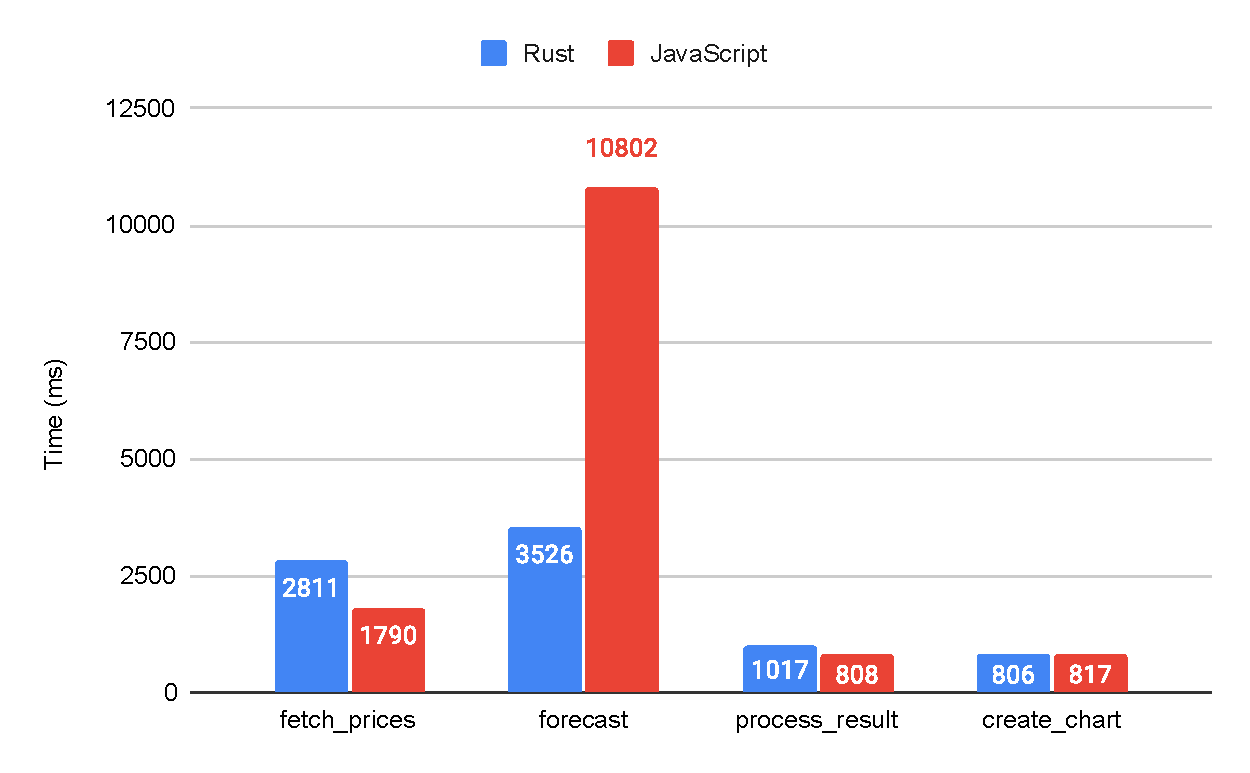
\includegraphics[width=\textwidth, keepaspectratio]{./assets/evaluation-language}
  \caption{Median Time spent per Language}
  \label{fig:time_per_language}
\end{figure}

As can be seen in \cref{fig:time_per_language}, for most function deployments,
the JavaScript version is faster or minimally slower than the Rust version.
In the cases where JavaScript is faster, the functions are really light-weight and
mostly only consist of a couple API calls and some basic logic in-between. We assume
that there exists a steady supply of JavaScript containers which are already
running while Rust containers have to be started first. When we look at the \texttt{forecast}
function, however, we see that the Rust version is considerably faster. This function
makes quite a few API calls and additionally transforms a JSON document into CSV. In
the Rust function, this is done in-memory, while the JavaScript function
saves the CSV to a file before uploading, which might explain why the Rust version
is faster in this case.

Another remark here has to be made to clarify that the numbers in \cref{tab:benchmark}
are for cached results, meaning the \texttt{forecast} function was run previously
and the forecast does not have to be done from scratch. Creating a forecast from
scratch can take from 45 minutes to 1 hour and 30 minutes. This means that first of all,
the deployed function will time out in any case since the maximum runtime of a function
on IBM Cloud is 10 minutes, and secondly, the difference between \texttt{forecast} runs can be up
to 45 minutes, which makes benchmarking them meaningless.

\begin{figure}[h]
  \centering
  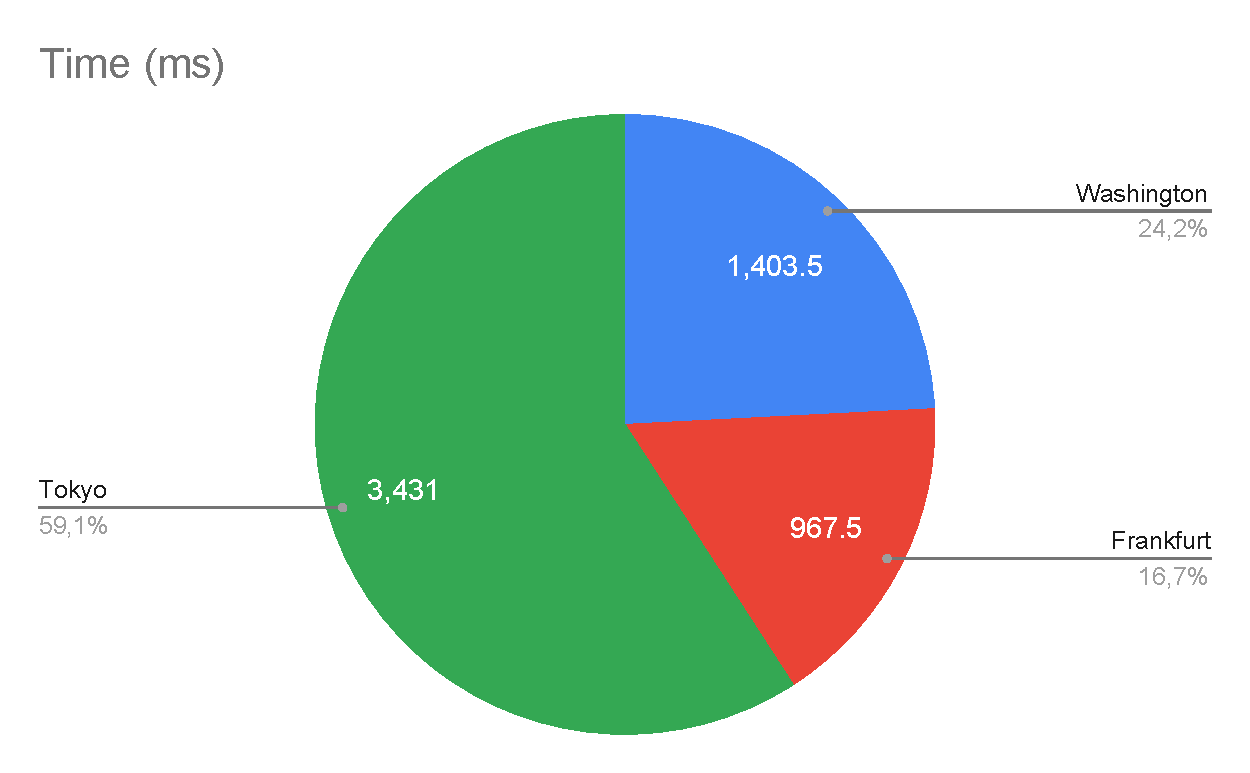
\includegraphics[width=\textwidth, keepaspectratio]{./assets/evaluation-region}
  \caption{Median Time spent per Region}
  \label{fig:time_per_region}
\end{figure}

In \cref{fig:time_per_region}, we see the median time across all functions in a region.
The difference between regions is expected. The benchmark was conducted from Austria,
so it was expected that the Frankfurt region would yield the fastest times. The only outlier
seems to be the JavaScript version of the \texttt{forecast} function in Frankfurt, which
takes longer than the same function in Washington. We could not come up with any
reasonable explanation why this might be the case.

Overall, the results show that once the forecast is cached, the complete function choreography
can be completed in approximately 20 seconds. Of course, if there is no cached result yet,
the enactment engine would have to retry for about an hour until it succeeds. In theory this
would work, but in practice it is probably more efficient to execute such a long-running process
in a VM.
